\begin{figure}[H]
  \begin{center}
    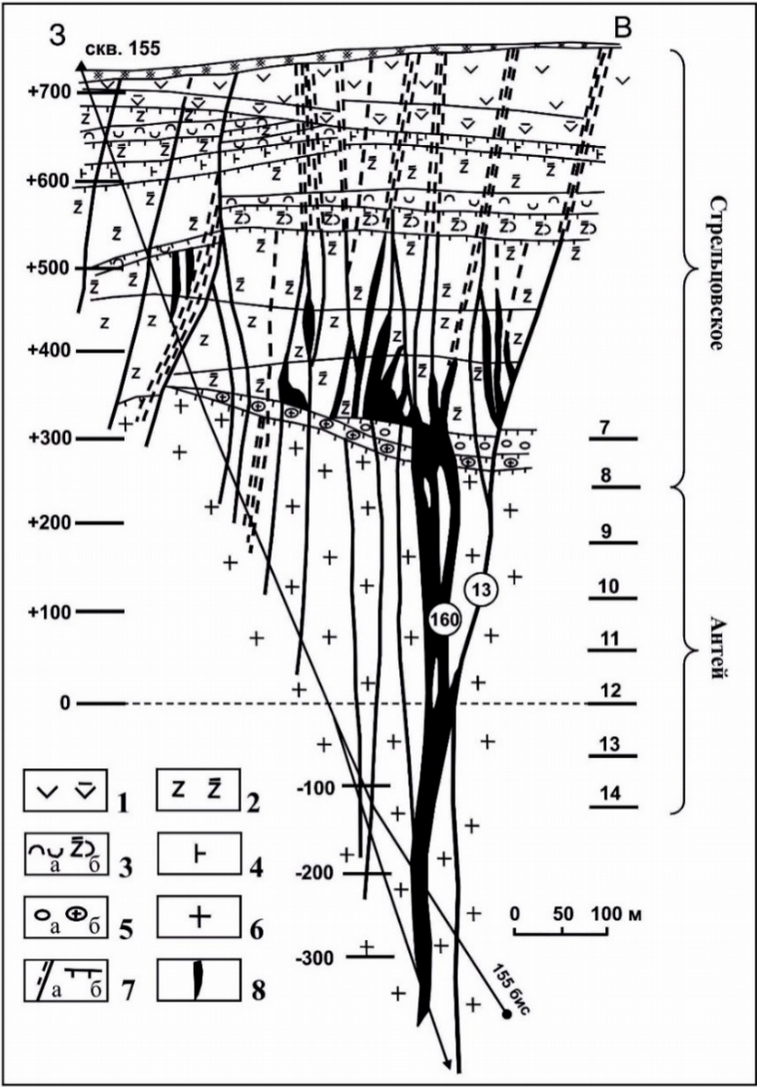
\includegraphics[width=0.75\textwidth]{authors/mandzhieva-fig-2.png}
  \end{center}
  \caption{Разрез по месторождениям Стрельцовское и Антей [5].
Условные обозначения: 1~--- фельзиты; 2~--- трахидациты; 3~--- туфы (а) и туфолавы (б) трахидацитов; 4~--- базальты; 5~--- конгломераты (а) и структурный элювий гранитов (б); 6~--- гранитоиды; 7~--- крутопадающий разлом (а) и пологие срывы (б); 8~--- рудные зоны и отдельные тела. Слева~--- шкала высот над уровнем моря, справа~--- положение в разрезе и номера горизонтов горных выработок}
  \label{fig:mandzhieva-fig2}
\end{figure}
